\documentclass[border=0pt]{standalone}

\usepackage{enumitem}

\usepackage[sc]{mathpazo}
\usepackage{tikz}
\linespread{1.05}

\newcommand\bluebullet{%
  \tikz[baseline=0ex]\fill[blue!75!black]
    (0,0)--(0.18,0.09)--(0,0.18)--cycle;}


\usepackage[table]{xcolor}
\definecolor{petrol}{RGB}{127,173,198}


\usepackage{tikz}
\usetikzlibrary{calc}


\usepackage{ragged2e}

\begin{document}
\small

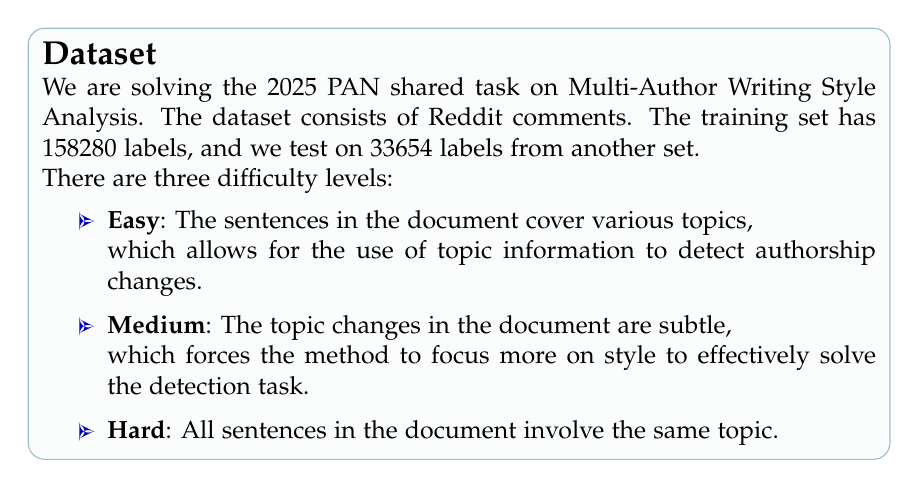
\begin{tikzpicture}
\node[
  draw=petrol!80,              
  fill=petrol!3,              
  rounded corners=6pt,
  minimum width=0.1\linewidth, 
  inner sep=5pt,               
  text width=0.92\linewidth-16pt, 
  font=\small,
  align=justify                
] (cap) {%
  \noindent {\large\textbf{Dataset}}\\
  \noindent We are solving the 2025 PAN shared task on Multi-Author Writing Style Analysis. The dataset consists of Reddit comments. The training set has 158280 labels, and we test on 33654 labels from another set.\\
 \noindent There are three difficulty levels:
\begin{itemize}[label=\bluebullet,left=1.5em,itemsep=3pt]
\item \textbf{Easy}: The sentences in the document cover various topics,\\which allows for the use of topic information to detect authorship changes.
\item \textbf{Medium}: The topic changes in the document are subtle,\\which forces the method to focus more on style to effectively solve the detection task.
\item \textbf{Hard}: All sentences in the document involve the same topic.
\end{itemize}
  };
\end{tikzpicture}

\end{document}